% !TEX root = 99_main.tex

%Cozie is built as a clock-face for fitbit, a wearable health tracker with 25 million active users \cite{fibit2018}. The application is publicly available for download at the following link [insert link]

\subsection{Overview}

The SDE Learning Trail framework describes NZEB's six different building features - Net Zero Energy, Water, Hybrid Cooling, Wellness, Tropical Architecture, and Biophilic Design - as distinct ‘trails’ for occupants and building visitors. Each ‘trail’ is composed of a number of physical 'stations' - in the form of QR codes - placed in close proximity of each other such that they help break down and explain a building feature in more detail.\\

The framework is realised as a simple mobile web application which connects each station (QR code) with information and interactive visualizations online, as shown in the Figure below \ref{fig:framework}. As occupants and visitors complete each trail by visiting different stations, the application collects comfort feedback for thermal, visual and aural variables while enabling them to learn and appreciate the design, construction, and sustainability features of the new NZEB.\\

\begin{figure}
\begin{center}
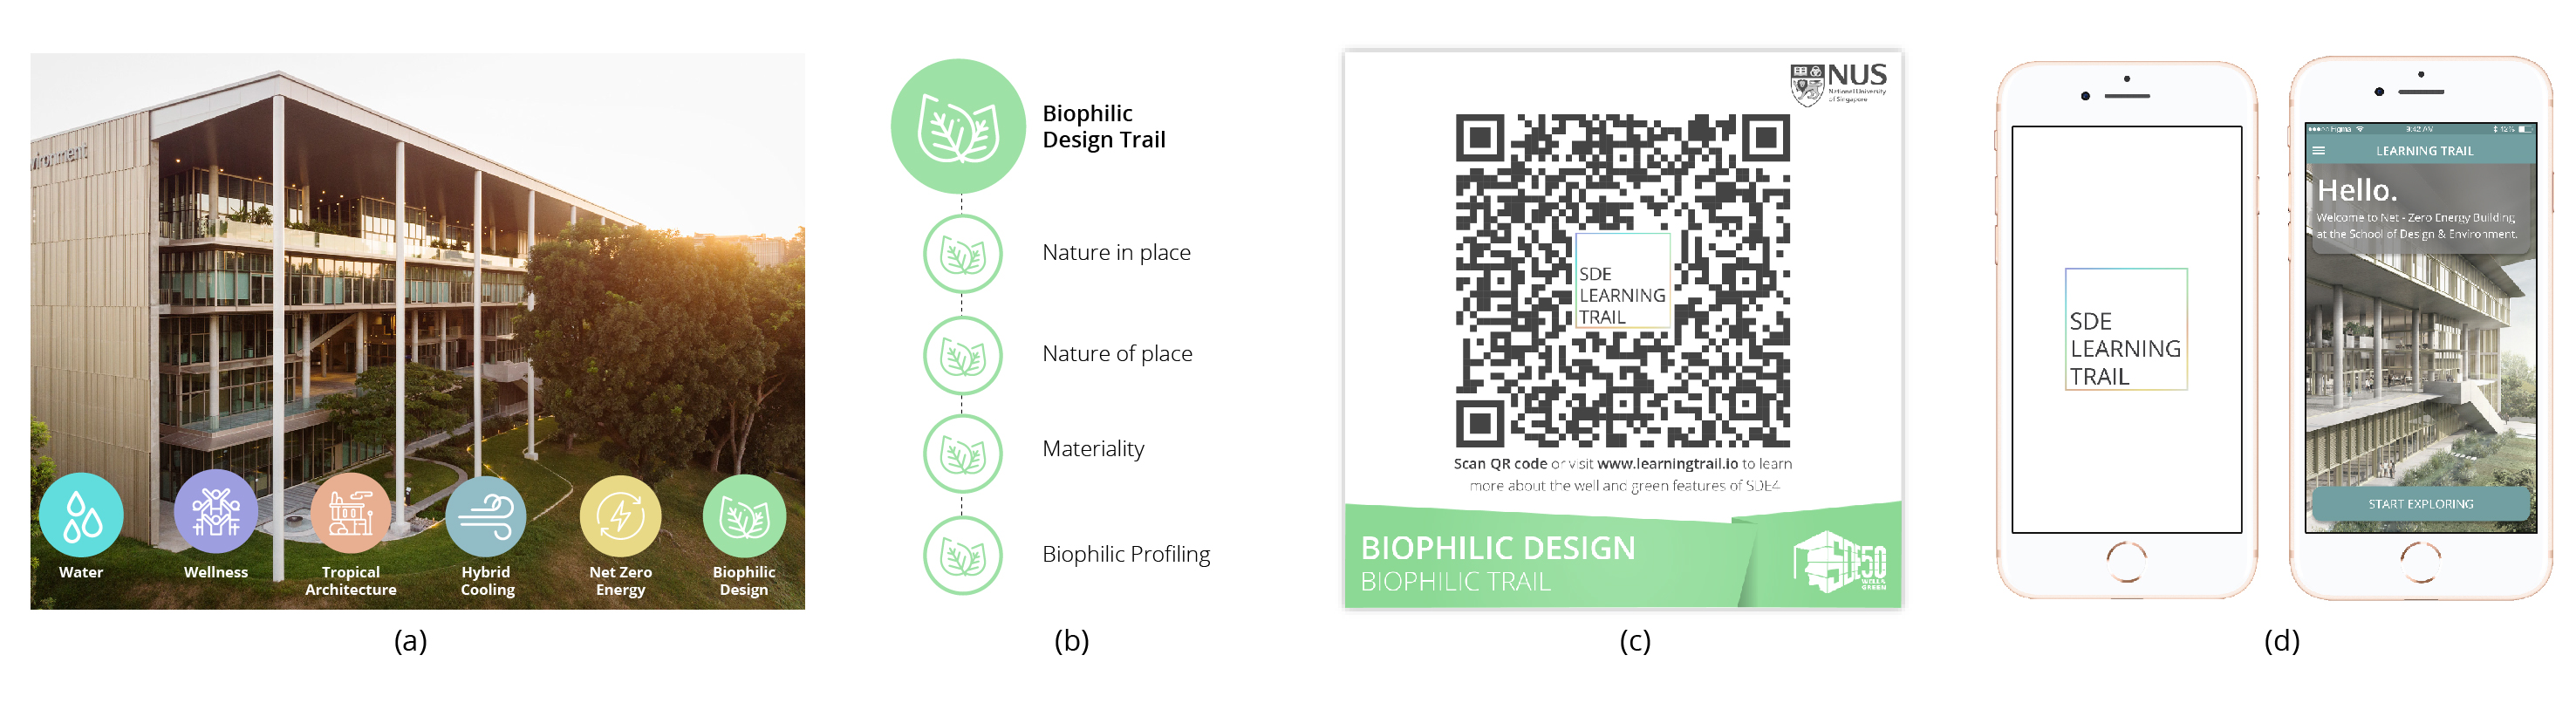
\includegraphics[width=\textwidth, trim= 0cm 0cm 0cm 0cm,clip]{Fig1.jpg}
\caption{Overview of SDE Learning Trail. (a) Building features described as trails, (b) Stations for Biophilic design trail (c) Digitisation of each station as a QR code, (d) Mobile web application.}
\label{fig:framework}
\end{center}
\end{figure}


% \begin{itemize}
%   \item Thermal: Prefer Warmer - Prefer Cooler
%   \item Light: Prefer brighter - Prefer Dimmer
%   \item Noise: Prefer Louder - Prefer Quieter 
%   \item Mood: Good - Neutral - Not So Good
%   \item Location: Indoor - Outdoor
%   \item Location: In Office - Out of Office
% \end{itemize}

%These responses will be grouped with the afore mentioned data, and stored in the Influx time series database. The manager is invited to contact the authors if they have further tailored questions that they would like to add.\\

%The watch-face also has the ability to prompt the user with a 3 second vibration, and force them to provide comfort feedback. This may be triggered at certain hours of the day, random hours of the day, at set time intervals, or at each 1000 steps walked. 

% \begin{figure}
%     \begin{subfigure}[t]{0.3\textwidth}
%         \includegraphics[height= 7cm]{iphone.png}
%     \end{subfigure}
%     \begin{subfigure}[t]{0.3\textwidth}
%         \includegraphics[height= 3cm]{flow.png}
%     \end{subfigure}
%     \caption{Using the fitbit mobile application to design a survey flow}
%     \label{fig:homescreen}
% \end{figure}




% \subsection{Building Data Labeling}

% The human comfort feedback can be combined with building sensor data to create a labeled data set of the environment. (perhaps talk more or delete this section)

% An example of this in practice will be introduced in the next section.